\subsection{Publication Step}

After the preparation step, which takes place on the desktop side, the RDFa enriched content is sent to the server via another REST call. The publication step of the process only handles public data. When the content is received it is parsed and the server extracts the contained RDF triples and stores them in its repository. The content (as it is received) is also stored.

The server implementation uses ARC2\footnote{\url{http://arc.semsol.org}}, as it provides out of the box RDFa parsing and an RDF repository. It is easily deployable due its minimal setup requirements (a PHP enabled Web server and a MySQL database), thus making our system easily deployable as well.

All server URIs are dereferenceable, as required by the Linked Data principles. For notes, the URI redirects to the RDFa annotated HTML page containing the note itself (as shown in Figure \ref{fig:views} (i)), the URI of the note being the URL of this page. For the linked resources, the URI is also dereferenceable and provides RDFa information about itself, linking to the known existing Web aliases of the same resource. The description also includes a list of backlinks to all the notes that reference the resource (see Figure \ref{fig:views} (ii)). The page for a tag will contain backlinks to all the notes tagged with it.

The RDFa annotated page for the note is generated on the user's desktop by the SemNotes plugin, as we have seen in the previous step, while the page describing each resource and tag is generated on the fly, by the server, when the URI is requested.

\begin{figure}[tb]
\begin{minipage}[b]{0.49\linewidth}
\begin{flushleft}
    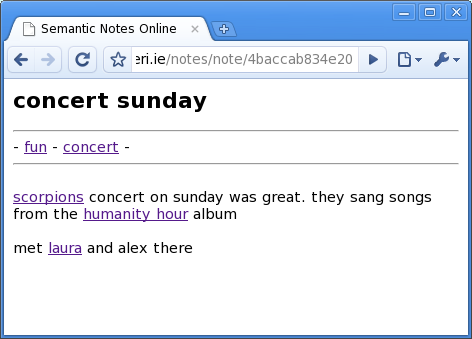
\includegraphics[width=0.97\linewidth]{chapters/core/img/noteview}
\end{flushleft}
\end{minipage}
\begin{minipage}[b]{0.49\linewidth}
\begin{flushright}
    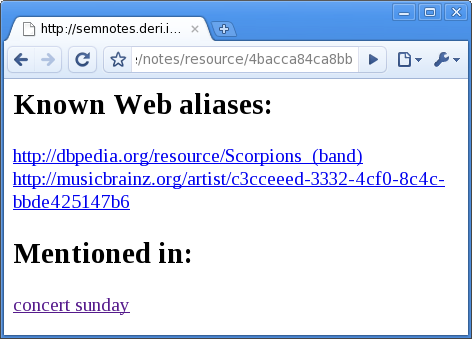
\includegraphics[width=0.97\linewidth]{chapters/core/img/resourceview}
\end{flushright}
\end{minipage}
\caption{Online view of a note (i) and a resource (ii).}
\label{fig:views}
\end{figure}
